
\item Hallar el mínimo de la función $f:(0,+\infty)\to \R$ dada por $\D f(x) = x + \frac1x$.

\item Hallar el punto de la parábola $y=x^2$ que está más cerca del punto $(3,0)$.

\item Hallar las dimensiones del cilindro circular recto de volumen $V$ que tenga mínima área exterior. (Si el cilindro tiene base circular de radio $r$ y altura $h$, entonces el volumen es: $\pi \, r^2\, h$ y el área exterior es $2\pi \, r^2 + 2 \pi \, r\, h$).

\item Consideremos la función $(x-1)^2+(x-2)^2+(x-6)^2$. Graficarla en Geogebra, y encontrar el valor mínimo y el punto mínimo.

\item Dados $a_1<a_2<\dots <a_n$, hallar el valor de $x$ que minimiza $\sum_{i=1}^n (a_i-x)^2$.

\item La siguientes figuras muestran la gráfica de \emph{la derivada $f'$ de $f$}. Hallar:
\begin{itemize}
  \item Todos los puntos máximos y mínimos locales de $f$.
  \item Intervalos de crecimiento y decrecimiento de $f$.
  \item Intervalos de convexidad y concavidad de $f$, y puntos de inflexión.
\end{itemize} 

\begin{multicols}{2}
  \begin{enumerate}
    \item 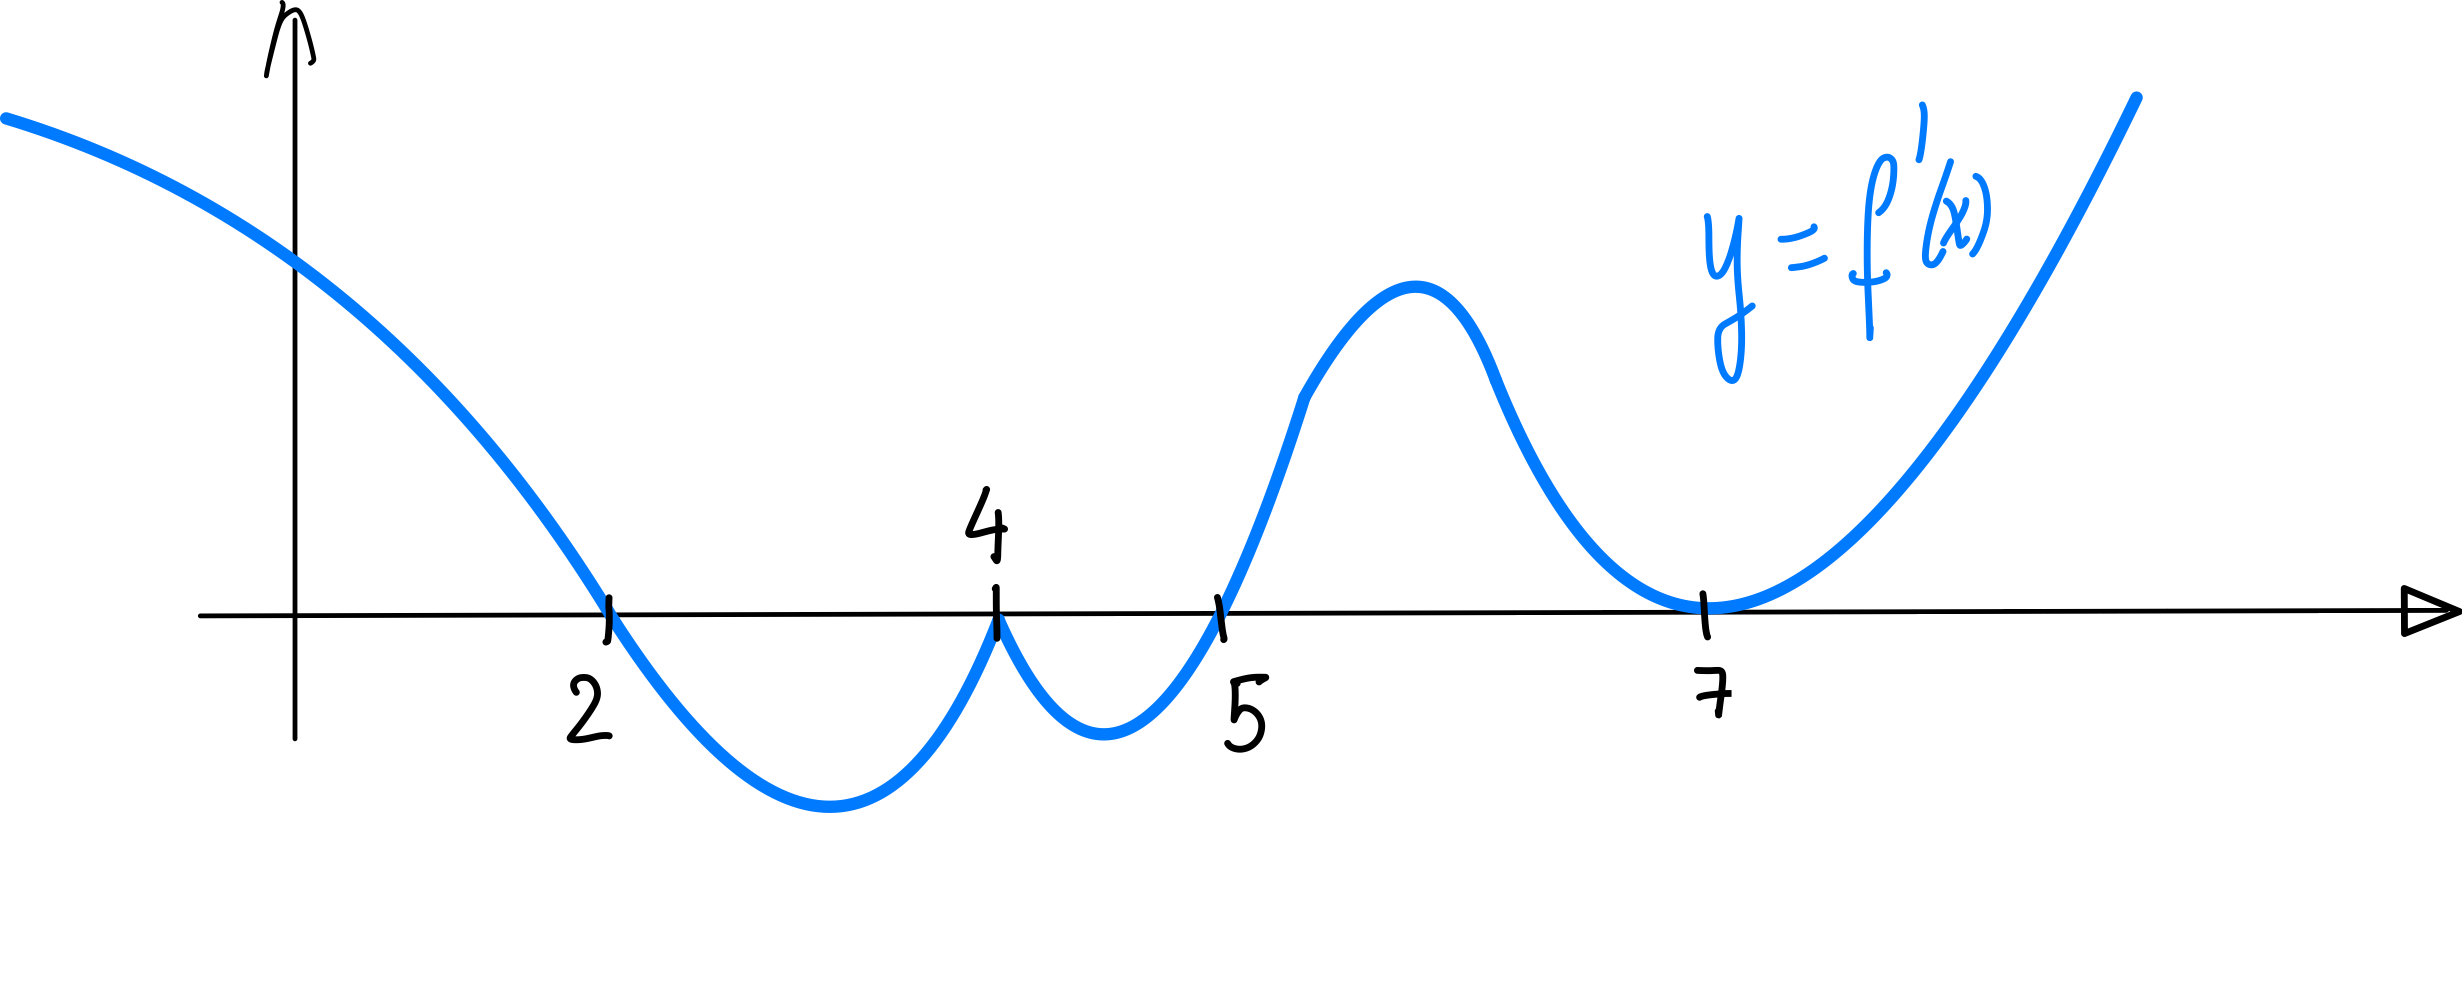
\includegraphics[width=.4\textwidth]{pics/max-min-locales-ej-a.png}
    \item 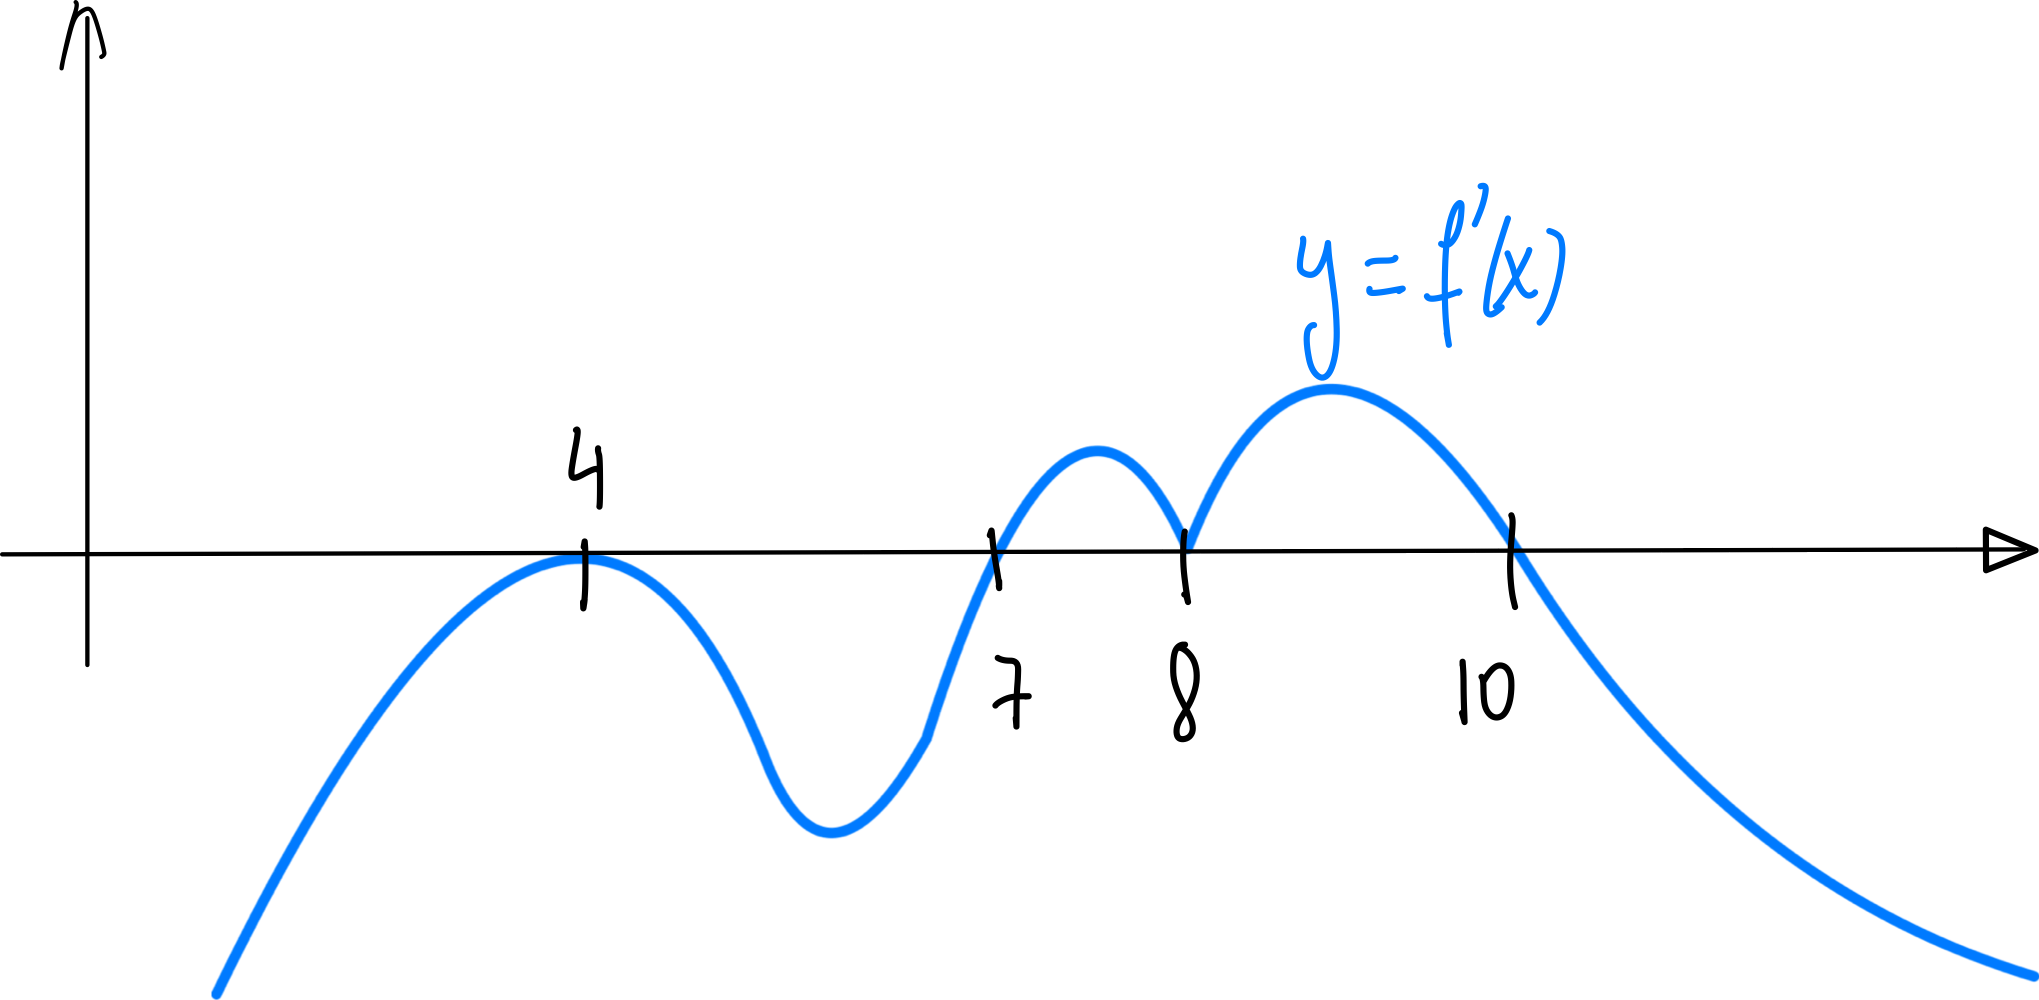
\includegraphics[width=.4\textwidth]{pics/max-min-locales-ej-b.png}
    \item 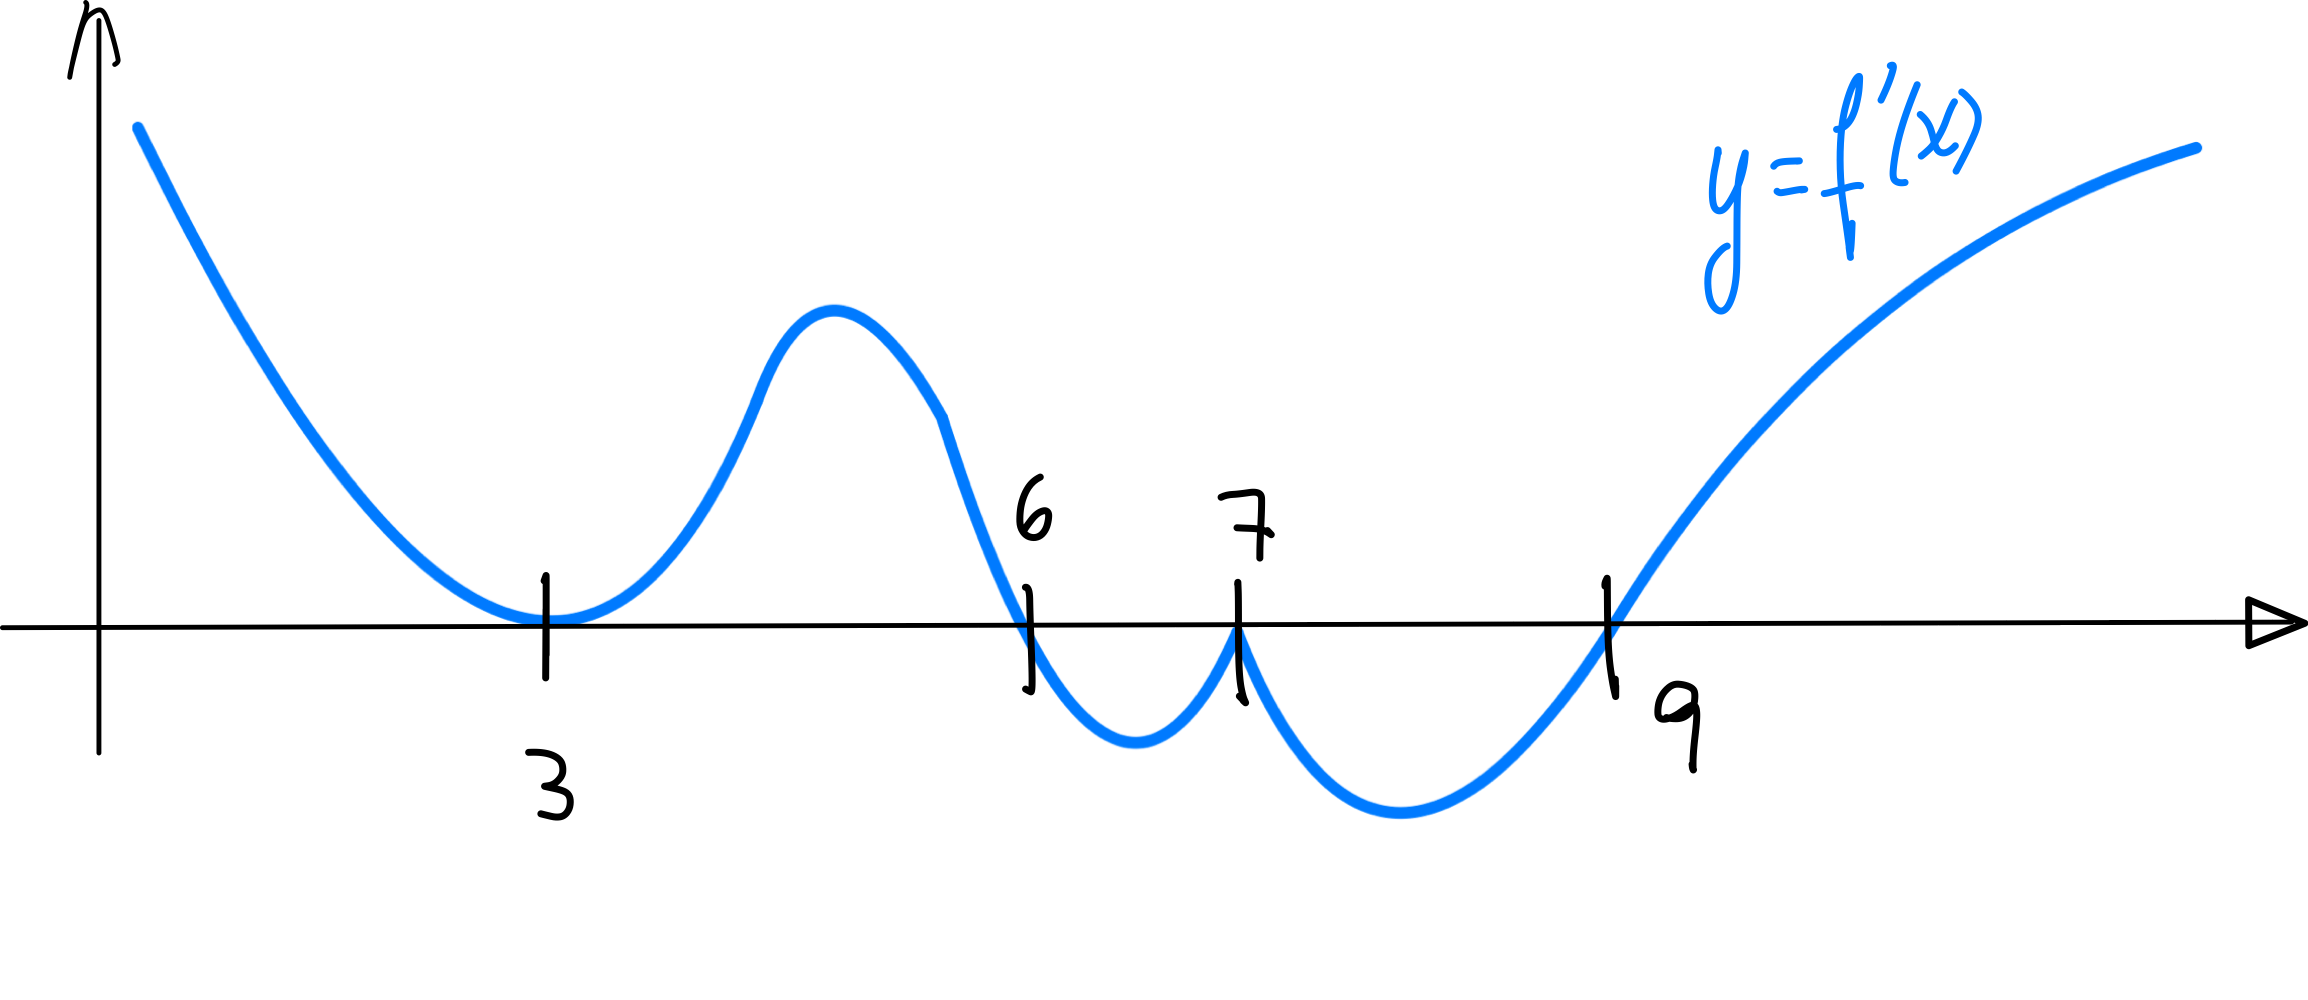
\includegraphics[width=.4\textwidth]{pics/max-min-locales-ej-c.png}
    \item 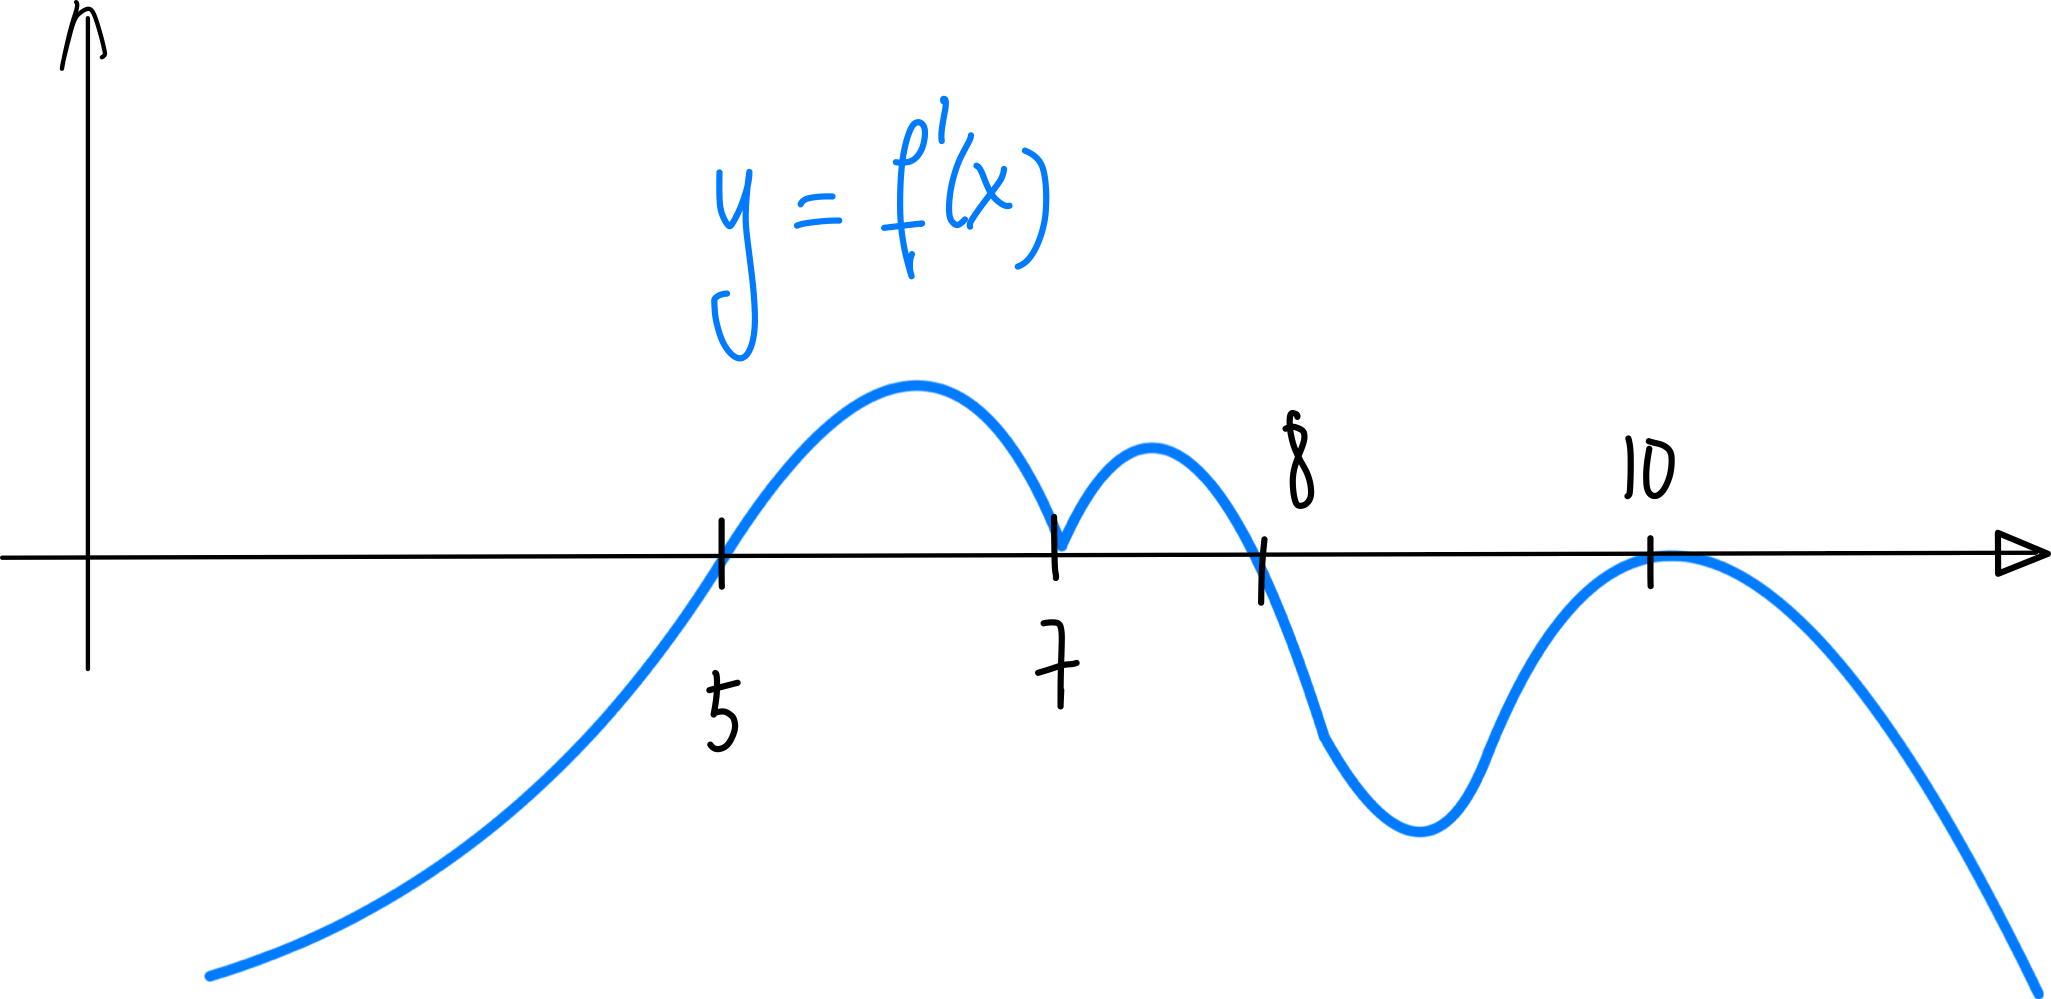
\includegraphics[width=.4\textwidth]{pics/max-min-locales-ej-d.png}
  \end{enumerate}
  
\end{multicols}
